% -*-latex-*-

\chapter{Uncertainty Estimation for Target Field Map}
\label{A2}

E08-027 uses a 2.5 Tesla (5.0 T in some configurations) magnetic field to polarize the ammonia target. The map of this magnetic field is used to trace the trajectory of the out-going electrons and reconstruct the kinematics of them. So the uncertainty of the field map becomes an important contribution to the final uncertainty of the kinematics. The target field is generated by a pair of super-conducting Helmholtz coils and the field map of these coils is calculated directly from the Biot-Savart law. To estimate the uncertainty of the calculation, a measurement of the target field is performed during the experiment. In this section we will summarize the measurement and give an estimation of the uncertainty of the field map.

\section{Target Field Measurement}
\label{A2S1}

The Hall effect is commonly used to measure magnetic field. It is difficult to place a Hall probe inside the target chamber so the field is measured several different positions on the surface of the target chamber. As shown in \cref{A2S1F1}, an aluminum block is used to keep a single-axis Hall probe perpendicular to the surface of the target chamber. The sensitive direction of the probe is the axial direction so it measures the $\hat{r}$-component of the target field in a cylindrical coordinate system. The origin of this coordinate system is the target center and the $\hat{h}$ is vertical up. Another Hall probe is also installed in the holder with the sensitive direction pointing to the azimuth direction to measure the $\hat{\phi}$-component of the target field. The position of each measuring point is surveyed in the HCS (See \Cref{C6S1SS1} for the definition of HCS). Once the coordinates is known, the theoretical values of $\Br$ and $\Bphi$ for each measuring point can be interpolated from the field map and compare with data.

\begin{figure}[tb!]
  \setlength{\unitlength}{1mm}
  \centering
  \begin{picture}(100,40)
    \thicklines
    \put(30,20){\circle{40}}
    \put(49.365,25){\line(1,0){6.76}}
    \put(49.365,15){\line(1,0){6.76}}
    \put(56,15){\line(0,1){10}}
    \put(49.365,25){\line(3,-1){4}}
    \put(49.365,15){\line(3,1){4}}
    \put(53.3,16.265){\line(0,1){7.5}}
    \put(51,19.75){\framebox(15,0.5){}}
    \put(30,20){\makebox(0,0){Chamber}}
    \put(62,31){\vector(-1,-1){5}}
    \put(63,32){\makebox(0,0)[lb]{Block}}
    \put(60,11){\vector(0,1){7}}
    \put(60,10){\makebox(0,0)[t]{Hall Probe}}
    \put(70,20){\vector(1,0){5}}
    \put(75,20){\makebox(0,0)[l]{$\Br$}}
    \put(70,20){\vector(0,1){5}}
    \put(70,25){\makebox(0,0)[b]{$\Bphi$}}
  \end{picture}
  \caption[Setup for target field mapping.]{Setup for target field mapping. The azimuth direction Hall probe is not shown in this figure. \label{A2S1F1}}
\end{figure}

\begin{table}[b!]
  \centering
  \begin{tabular}{|*{6}{c|}}
    \hline
    Probe & $r_0$/mm & $\phi_0$/rad & $h_0$/mm & $\theta$/rad & $\phi$/rad \\ \hline
    $r$    & 10.74 & 0.1351 &  0.00 & 0.0983 & 3.5197 \\ \hline
    $\phi$ & 16.17 & 0.1351 & -4.01 & 1.5032 & 3.1346 \\ \hline
  \end{tabular}
  \caption[Fit result of the offset of the Hall probes.]{Fit result of the space offset and angle deviation of the Hall probes. $r_0$, $\phi_0$, $h_0$ are in the cylindrical coordinate system of the target chamber. $\theta$ and $\phi$ are azimuth angles with respect to the $\hat{r}$ direction. \label{A2S1T1}}
\end{table}

The readout of the Hall probes need to be calibrated first since the sensitive direction of the probe may not align to the radial direction and azimuth direction perfectly. Mechanical errors can arise from the installation of the Hall probe into the aluminum holder, and cause some space deviation between the actual sensitive point of the probe and surveyed coordinates of the measuring point. Thus, the probe is considered to have five degrees of freedom: a space offset ($r_0$, $\phi_0$, $h_0$) with respect to the measuring point and an angle deviation ($\theta$, $\phi$) with respect to the local $\hat{r}$ direction. The readout of the probes should be projected to the actual $\hat{r}$ and $\hat{\phi}$ direction to extract the measured values of $\Br$ and $\Bphi$. However, the space offset ($r_0$, $\phi_0$, $h_0$) and the angle deviation ($\theta$, $\phi$) of the probe is very difficult to be directly measured without destroying the probe. Thus, the probe readout is used to fit $\Br$ and $\Bphi$. In the fit, ($r_0$, $\phi_0$, $h_0$) and ($\theta$, $\phi$) are treated as free parameters to minimize the difference between the theoretical values of $\Br$ and $\Bphi$ and their measured values. The fit result is shown in \cref{A2S1T1}. Once the parameters is fixed by the fit, the measured values of $\Br$ and $\Bphi$ and their theoretical values are listed in \cref{A2S1T2}. \Cref{A2S1F2} shows the differences between the measured value and the theoretical value from the field map. The average deviation between the measurement and the field map is 4.7 gauss for $\Br$ and 4.4 gauss for $\Bphi$.

\begin{figure}[tb!]
  \centering
  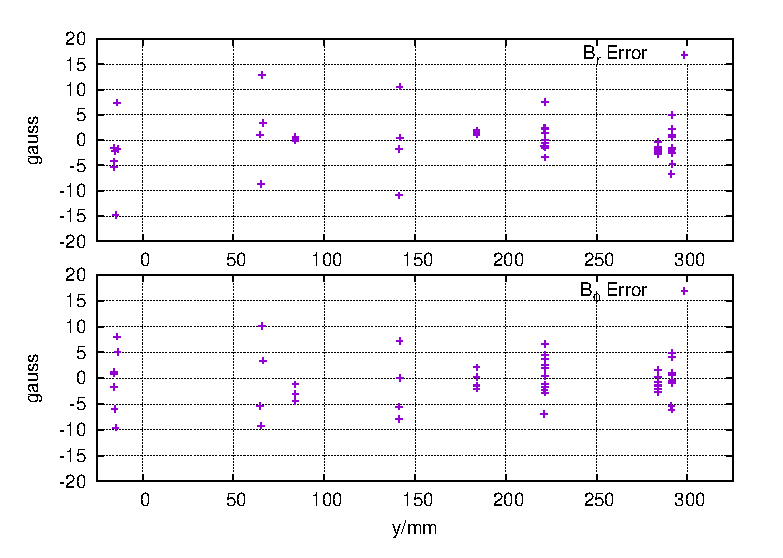
\includegraphics[width=0.75\textwidth]{figs/target-field-mapping-error}
  \caption{The differences between the measured field and the map. \label{A2S1F2}}
\end{figure}

\begin{center}
  \singlespacing
  \tablefirsthead{%
    \hline
    ID & $x$/mm & $y$/mm & $z$/mm & $\Br^{\text{data}}$ & $\Br^{\text{map}}$ & $\Br^{\text{error}}$ & $\Bphi^{\text{data}}$ & $\Bphi^{\text{map}}$ & $\Bphi^{\text{error}}$ \\ \hline
  }
  \tablehead{%
    \hline
    \multicolumn{10}{|l|}{\small\sl continued from previous page}\\ \hline
    ID & $x$/mm & $y$/mm & $z$/mm & $\Br^{\text{data}}$ & $\Br^{\text{map}}$ & $\Br^{\text{error}}$ & $\Bphi^{\text{data}}$ & $\Bphi^{\text{map}}$ & $\Bphi^{\text{error}}$ \\
  }
  \tabletail{%
    \hline
    \multicolumn{10}{|r|}{\small\sl continued on next page}\\ \hline
  }
  \tablelasttail{\hline}
  \bottomcaption[Compare between the measured field and the field map.]{Compare between the measured field and the field map. The unit of fields are gauss. \label{A2S1T2}}
  \begin{supertabular}{|*{10}{c|}}
     1 &   414.08 &   283.78 &  -242.54 &   -433.0 &   -432.6 &     -0.4 &   -460.8 &   -462.4 &      1.6 \\ \hline
     2 &   386.75 &   283.78 &  -284.15 &   -486.8 &   -485.2 &     -1.6 &   -430.5 &   -429.1 &     -1.4 \\ \hline
     3 &   355.26 &   283.77 &  -322.71 &   -534.5 &   -531.7 &     -2.8 &   -389.1 &   -389.3 &      0.2 \\ \hline
     4 &   319.94 &   283.78 &  -357.79 &   -572.4 &   -571.1 &     -1.3 &   -346.5 &   -344.5 &     -2.0 \\ \hline
     5 &   281.17 &   283.78 &  -389.02 &   -605.5 &   -603.1 &     -2.4 &   -299.1 &   -296.4 &     -2.7 \\ \hline
     6 &   239.38 &   283.79 &  -416.07 &   -629.4 &   -627.5 &     -1.9 &   -246.8 &   -246.1 &     -0.7 \\ \hline
     7 &   413.92 &   183.93 &  -242.65 &   -720.9 &   -722.4 &      1.5 &   -599.2 &   -597.2 &     -2.0 \\ \hline
     8 &   386.58 &   183.92 &  -284.25 &   -812.1 &   -813.2 &      1.1 &   -553.8 &   -552.4 &     -1.4 \\ \hline
     9 &   355.08 &   183.92 &  -322.80 &   -889.1 &   -890.9 &      1.8 &   -498.1 &   -498.3 &      0.2 \\ \hline
    10 &   319.75 &   183.92 &  -357.87 &   -952.2 &   -954.1 &      1.9 &   -436.3 &   -438.4 &      2.1 \\ \hline
    11 &   413.76 &    84.08 &  -242.75 &  -1004.0 &  -1004.2 &      0.2 &   -707.7 &   -703.2 &     -4.5 \\ \hline
    12 &   386.41 &    84.07 &  -284.35 &  -1128.8 &  -1129.4 &      0.6 &   -649.5 &   -646.5 &     -3.0 \\ \hline
    13 &   354.90 &    84.07 &  -322.89 &  -1232.3 &  -1232.2 &     -0.1 &   -579.9 &   -578.7 &     -1.2 \\ \hline
    14 &   413.60 &   -15.77 &  -242.86 &  -1108.2 &  -1106.6 &     -1.6 &   -732.2 &   -730.5 &     -1.7 \\ \hline
    15 &   386.24 &   -15.78 &  -284.45 &  -1247.6 &  -1243.4 &     -4.2 &   -668.9 &   -669.8 &      0.9 \\ \hline
    16 &   354.72 &   -15.78 &  -322.98 &  -1359.4 &  -1354.0 &     -5.4 &   -596.3 &   -597.6 &      1.3 \\ \hline
    17 &   210.61 &   221.61 &  -431.32 &   -896.8 &   -893.4 &     -3.4 &   -248.0 &   -250.0 &      2.0 \\ \hline
    18 &   164.78 &   221.57 &  -450.84 &   -910.4 &   -909.8 &     -0.6 &   -194.0 &   -191.2 &     -2.8 \\ \hline
    19 &   117.17 &   221.54 &  -465.51 &   -918.7 &   -917.6 &     -1.1 &   -130.2 &   -132.8 &      2.6 \\ \hline
    20 &    68.30 &   221.51 &  -475.15 &   -915.9 &   -917.3 &      1.4 &    -75.9 &    -74.3 &     -1.6 \\ \hline
    21 &    18.69 &   221.49 &  -479.67 &   -906.7 &   -908.9 &      2.2 &    -11.5 &    -15.2 &      3.7 \\ \hline
    22 &   -31.12 &   221.46 &  -479.03 &   -892.3 &   -892.4 &      0.1 &     49.5 &     44.9 &      4.6 \\ \hline
    23 &   -80.59 &   221.43 &  -473.22 &   -868.7 &   -867.2 &     -1.5 &    107.0 &    106.6 &      0.4 \\ \hline
    24 &   210.61 &   291.67 &  -431.36 &   -614.8 &   -610.1 &     -4.7 &   -208.3 &   -207.9 &     -0.4 \\ \hline
    25 &   164.78 &   291.63 &  -450.87 &   -623.8 &   -622.3 &     -1.5 &   -157.8 &   -157.2 &     -0.6 \\ \hline
    26 &   117.17 &   291.60 &  -465.53 &   -630.5 &   -627.9 &     -2.6 &   -107.0 &   -106.0 &     -1.0 \\ \hline
    27 &    68.30 &   291.57 &  -475.17 &   -628.8 &   -627.2 &     -1.6 &    -55.0 &    -54.5 &     -0.5 \\ \hline
    28 &    18.69 &   291.54 &  -479.68 &   -617.8 &   -620.1 &      2.3 &     -1.9 &     -2.5 &      0.6 \\ \hline
    29 &   -31.12 &   291.52 &  -479.03 &   -606.1 &   -606.7 &      0.6 &     54.3 &     50.2 &      4.1 \\ \hline
    30 &   -80.60 &   291.49 &  -473.21 &   -588.4 &   -586.7 &     -1.7 &    108.3 &    103.4 &      4.9 \\ \hline
    31 &  -142.22 &   291.61 &  -458.45 &   -549.9 &   -550.9 &      1.0 &    172.7 &    171.7 &      1.0 \\ \hline
    32 &  -229.55 &   291.45 &  -421.51 &   -472.6 &   -477.6 &      5.0 &    273.2 &    272.3 &      0.9 \\ \hline
    33 &  -315.51 &   291.28 &  -361.60 &   -372.0 &   -369.8 &     -2.2 &    365.1 &    371.2 &     -6.1 \\ \hline
    34 &  -371.09 &   291.13 &  -304.21 &   -281.5 &   -274.8 &     -6.7 &    424.0 &    429.3 &     -5.3 \\ \hline
    35 &  -142.04 &   221.61 &  -458.52 &   -818.3 &   -820.7 &      2.4 &    185.9 &    187.1 &     -1.2 \\ \hline
    36 &  -229.39 &   221.45 &  -421.63 &   -712.9 &   -720.4 &      7.5 &    316.8 &    310.1 &      6.7 \\ \hline
    37 &  -315.38 &   221.28 &  -361.77 &   -562.0 &   -564.4 &      2.4 &    432.9 &    435.1 &     -2.2 \\ \hline
    38 &  -370.99 &   221.13 &  -304.40 &   -422.9 &   -421.7 &     -1.2 &    501.7 &    508.6 &     -6.9 \\ \hline
    39 &  -141.83 &   141.61 &  -458.61 &  -1148.9 &  -1149.4 &      0.5 &    196.3 &    196.3 &      0.0 \\ \hline
    40 &  -229.21 &   141.45 &  -421.76 &  -1013.6 &  -1024.2 &     10.6 &    350.3 &    343.1 &      7.2 \\ \hline
    41 &  -315.23 &   141.28 &  -361.95 &   -824.5 &   -813.6 &    -10.9 &    491.6 &    499.5 &     -7.9 \\ \hline
    42 &  -370.88 &   141.13 &  -304.62 &   -612.3 &   -610.5 &     -1.8 &    586.8 &    592.3 &     -5.5 \\ \hline
    43 &  -141.84 &    66.23 &  -458.62 &  -1385.2 &  -1388.6 &      3.4 &    202.5 &    199.1 &      3.4 \\ \hline
    44 &  -229.07 &    65.67 &  -421.87 &  -1238.9 &  -1251.8 &     12.9 &    371.0 &    360.9 &     10.1 \\ \hline
    45 &  -314.99 &    65.04 &  -362.22 &  -1015.3 &  -1006.6 &     -8.7 &    530.2 &    539.4 &     -9.2 \\ \hline
    46 &  -370.60 &    64.55 &  -305.04 &   -757.9 &   -759.0 &      1.1 &    641.6 &    647.0 &     -5.4 \\ \hline
    47 &  -141.67 &   -13.74 &  -458.69 &  -1472.7 &  -1470.9 &     -1.8 &    205.9 &    200.8 &      5.1 \\ \hline
    48 &  -228.93 &   -14.30 &  -421.98 &  -1321.8 &  -1329.2 &      7.4 &    374.2 &    366.1 &      8.1 \\ \hline
    49 &  -314.88 &   -14.93 &  -362.38 &  -1086.4 &  -1071.6 &    -14.8 &    540.3 &    549.9 &     -9.6 \\ \hline
    50 &  -370.51 &   -15.42 &  -305.23 &   -810.6 &   -808.5 &     -2.1 &    654.8 &    660.8 &     -6.0 \\
  \end{supertabular}
\end{center}

\section{Uncertainty Estimation}
\label{A2S2}

The average deviations between the measured fields and the field map have been calculated in \Cref{A2S1}. The value is close to 5 gauss around the target chamber. However, this result has assumed that the calibration of the orientation of the Hall probes is accurate. Since it is difficult to be verified with real measurement, this assumption may not be true. The influence of the orientation of the Hall probes to the uncertainty of the measured field can be estimated by adding an uncertainty of certain level to the azimuth angle of the probes and recalculate the average deviations between the measured fields and the predicted values from the field map. Two situations is tested here to estimate the uncertainty. If the azimuth angle of the probes is increased by 10 mrad, the average deviations increase to 6.71 gauss for $\Br$ and 10.18 gauss for $\Bphi$. If the azimuth angle of the probes is decreased by 10 mrad, the average deviations increase to 6.67 gauss for $\Br$ and 10.17 gauss for $\Bphi$. So it is safe for us to conclude that the uncertainty of this measurement is less than 12 gauss and the relative uncertainty is 1.2\% (the average field strength around the target chamber is $\sim$1000 gauss).

The angle deviation of a charged particle in a static magnetic field can be expressed by equation:
\begin{equation} \label{A2S2E1}
\Delta\theta=\frac{q}{mv}\int_{L}\vec{B}\times\dd{\vec{l}}.
\end{equation}
Here the integration is along the trajectory of the particle and the integrand is referred as the $\Bdl$ of the trajectory. Thus, the uncertainty of the target field need to be propagate to the integration of $\Bdl$ to give its contribution of the uncertainty of the kinematics variables. The uncertainty of the target field outside the target field has been estimated above. During the experiment, the field strength at the target center is monitored by NMR method. The relative uncertainty of this method is less than 0.1\%. The uncertainty of the target field in the other region of the target chamber is not known, so an interpolation between 0.1\% and 1.2\% will be used when applying \cref{A2S2E1}. The simulation package is used to calculate the integrated $\Bdl$. With a 2.5 T transverse target field, the integrated $\Bdl$ is $6.682\times 10^{-1}$ T$\cdot$m, and the uncertainty is $5.682\times 10^{-3}$ T$\cdot$m, the relative uncertainty is 0.85\%. Thus, the contribution of the uncertainty of the target field map to the scattering angle is about 0.85\%.

\newpage
\cleardoublepage

%%%%%%%%%%%%%%%%%%%%%%%%%%%%%%%%%%%%%%%%%%%%%%%%%%%%%%%%%%%%%%%%%%%%%%
% -*-latex-*-
